% !TeX program = xelatex
% Editable consolidated manuscript: all prose, tables, equations, and references are in this file.
% Keep the accompanying figures/ directory beside this file.
% Compile with XeLaTeX twice. No BibTeX/Biber or other source .tex files are required.
\documentclass[a4paper,11pt]{article}
\usepackage[english]{babel}
\usepackage[T1]{fontenc}
\usepackage{lmodern}
\usepackage[margin=2.35cm,headheight=14pt]{geometry}
\usepackage{amsmath,amssymb,bm,booktabs,tabularx,array}
\usepackage{graphicx,float,caption,enumitem,xcolor,fancyhdr}
\usepackage[numbers,sort&compress]{natbib}
\usepackage{hyperref,xurl,microtype}
\usepackage[section]{placeins}
\usepackage{needspace}
\definecolor{navy}{HTML}{17324D}
\definecolor{teal}{HTML}{287D8E}
\hypersetup{colorlinks=true,linkcolor=navy,citecolor=teal,urlcolor=teal,
 pdftitle={Auto-ORCA: An LLM-Guided Agent for Autonomous DFT Calculations},
 pdfauthor={CHEN GENG},pdflang={en}}
\urlstyle{same}
\graphicspath{{figures/}}
\renewcommand{\arraystretch}{1.18}
\setlength{\tabcolsep}{5pt}
\setlength{\emergencystretch}{3em}
\clubpenalty=10000
\widowpenalty=10000
\linespread{1.08}
\renewcommand{\topfraction}{0.9}
\renewcommand{\bottomfraction}{0.85}
\renewcommand{\textfraction}{0.08}
\renewcommand{\floatpagefraction}{0.8}
\setlist{nosep,leftmargin=2em}
\captionsetup{font=small,labelfont=bf,labelsep=period}
\pagestyle{fancy}
\fancyhf{}
\fancyhead[L]{\small Auto-ORCA}
\fancyfoot[C]{\thepage}
\newcolumntype{Y}{>{\raggedright\arraybackslash}X}
\newcommand{\Eh}{E_{\mathrm h}}
\newcommand{\code}[1]{\texttt{#1}}
\title{\vspace{-1.0cm}\LARGE\bfseries
 Auto-ORCA: An LLM-Guided Agent\\[0.2em]
 for Autonomous DFT Calculations}
\author{\large CHEN GENG}
\date{}
\begin{document}
\maketitle
\vspace{-0.7cm}
\begin{abstract}
  Molecular density functional theory (DFT) studies require coordination of structure preparation, electronic-structure calculations, result assessment, and subsequent calculations.
  This work presents Auto-ORCA, which connects large language models' task-planning and code-generation capabilities to a managed ORCA execution environment.
  Calculations share a unified ORCA entry point, and their outputs inform plan revisions.
  The system stores scientific objectives separately from execution plans, retrieves versioned domain information as needed, and links results to inputs, geometries, and raw outputs.
  Seven test cases examine geometry optimization and vibrational frequencies, candidate conformer energies, dihedral scans, vertical excitations, environmental effects, and response tensors.
  Defining success as the production of computational outputs for each test problem gives a success rate of $6/7$.
  Ethanol optimization converged with 21 positive frequencies and no imaginary frequencies; single-point energies were compared for six candidate geometries of \textit{n}-hexane; five singlet excitation energies were obtained for acetone; electronic-energy differences between CPCM water and the gas phase were $-18.276507$ and $-16.607972$ kJ mol$^{-1}$ with two basis sets; and complete shielding tensors were obtained for all three HCN nuclei.
  Six constrained optimization points were computed successfully for \textit{n}-butane, but their actual dihedral angles still require independent verification; formaldehyde polarizability values remain unavailable.
  These results support the feasibility of combining generic tools and generated code for diverse DFT tasks.
  Comprehensive conclusions about potential energy surfaces require further geometric validation and sampling evidence.
\end{abstract}

\section{Introduction}
Molecular structure, conformational stability, and reaction pathways are closely related to potential energy surfaces.
Density functional theory (DFT) uses the electron density as its fundamental variable, with the Kohn--Sham framework enabling practical electronic-structure calculations~\cite{hk,ks}.
Each calculation addresses a question only for a particular method, geometry, and environment.
A complete study must also organize geometry optimization, vibrational analysis, candidate comparison, and constrained scans, using intermediate results to guide subsequent actions.

Challenges often arise between computational steps.
Frequency analysis requires the correct optimized structure, candidate energies must correspond to specific geometries, and environmental comparisons must retain common computational conditions.
Where established protocols are insufficient, researchers must implement new sampling and analysis procedures.
Autonomous computational systems must therefore connect natural-language requirements, execution, and scientific evidence within an ongoing decision process, rather than merely generate an input file.

Auto-ORCA is built on ORCA and the ORCA Python Interface (OPI)~\cite{orca2020,orca6,opipaper}.
A single agent organizes task planning, code generation, and result interpretation, while generic tools handle input validation, computational execution, and artifact management.
Original objectives and minimum evidence requirements are stored independently of the plan, allowing execution strategies to change while preserving task-completion criteria.

The study asks three questions: whether generated code can express diverse molecular computation tasks, whether a unified execution entry point can produce actual numerical results, and how fully these results answer the original scientific questions.
Seven test problems with distinct operational requirements examine these capabilities.
Geometry optimization, conformer comparison, and dihedral scanning test operations related to potential energy surfaces; excited states, environmental effects, and response tensors assess the same computational mechanism's applicability to other properties.
The focus is on organizing and validating autonomous computation, without introducing a new electronic-structure approximation.
The design translates open-ended natural-language requirements into executable tasks, combines bounded task code with a unified ORCA entry point, and preserves correspondence among original objectives, computational evidence, and final reports.
These mechanisms aim to reduce repetitive operations, broaden task expressiveness, and improve result verifiability.

\section{Related Work and Motivation}
\subsection{From Traceable Workflows to Semantic Tool Composition}
Computational automation requires consistent execution interfaces and provenance records.
Independent verification depends on records of structure-file transfers, input conditions, the calculation that produced each output, and evidence retained after abnormal termination.
ASE connects different simulation programs through common atomic-structure and calculator interfaces; AiiDA links computational processes to data provenance; Atomate2 provides composable workflows for materials calculations; and cclib supports unified parsing of outputs from different quantum-chemistry packages~\cite{ase,aiida,atomate2,cclib}.
These approaches underpin structure transfer, task execution, and result verification.

Language models can then translate natural-language requirements into tool selections, parameters, and operational dependencies.
Specialized tools provide defined behavior, but new sampling procedures and cross-result analyses may require additional implementation.
Generated task code can express bounded loops, candidate selection, and deterministic analysis.
Fixed workflows, semantic tool composition, and code generation differ in their predefined content and runtime expressiveness; all require input validation and provenance tracking.

\subsection{Language-Model Agents and Task Code in a Closed Loop}
ReAct interleaves reasoning and action, using external observations to update subsequent operations; Toolformer investigates learned tool use; and Reflexion supports task revision through linguistic feedback~\cite{react,toolformer,reflexion}.
In chemistry, ChemCrow connects language models to specialist tools, while Coscientist explores model coordination of chemical research operations~\cite{chemcrow,coscientist}.
These studies indicate that models can interpret requirements and organize operations, but tool use still requires explicit inputs, inspectable outputs, and domain knowledge.

Syntactically correct ORCA input alone is insufficient for autonomous electronic-structure exploration.
An input describes a single calculation, whereas scientific tasks often comprise several interdependent calculations.
The origin of the initial geometry, the structure needed next, consistent conditions across energy values, and sufficient evidence to justify stopping all extend beyond an individual input file.
A closed-loop system must reassess these questions after each calculation and incorporate relevant outputs into subsequent decisions and plans.

Task code expresses this process flexibly.
A model can generate a bounded program combining geometry transformations, calculation requests, and result analysis, then use the returned artifacts to determine whether further operations are needed.
The central requirement is to link every internal calculation to the original objective, rather than simply generate a longer script.
For example, conformer-comparison programs must retain candidate geometries and energies to make rankings traceable to structures.
Scanning programs must preserve correspondence among target labels, optimized geometries, and actual dihedral angles.
Code represents the algorithm; calculation receipts and raw outputs provide execution evidence.

A program may contain several internal calculations, so a successful tool call does not establish that every subproblem has been answered.
Likewise, extracting a number does not establish that it represents the required physical quantity.
Auto-ORCA therefore expresses task algorithms through generated code while managing calculation conditions, resource consumption, and artifact provenance through a shared execution entry point, linking flexibility to verifiable execution records.

\subsection{Closed-Loop DFT Automation and System Design Choices}
AutoDFT targets VASP calculations, translating natural-language tasks and crystal structures into computational steps whose parameters are generated from existing results.
Its seven agent types distribute planning, execution, monitoring, repair, reflection, and property extraction; even converged results can trigger recalculation or plan adjustment, with properties ultimately produced through deterministic postprocessing~\cite{autodft}.

Auto-ORCA addresses these questions in molecular calculations and potential-energy-surface operations through a single agent's decision loop.
Intent recognition, planning, code generation, result assessment, and reporting are stages of the same decision process.
Tools define the execution boundary, ORCA performs electronic-structure calculations, and programmatic checks and raw evidence constrain interpretation.
This organization maintains objectives, conditions, and subsequent actions within a shared context, linking input structures, execution records, and final conclusions.

\subsection{Scientific Evidence and Scope of Evaluation}
Autonomous electronic-structure computation must distinguish calculation completion from satisfaction of a scientific objective.
Lee and Rondinelli's autonomous multireference quantum chemistry study distinguishes computational convergence from correspondence to the target electronic state~\cite{multirefagent}.
Here, this issue concerns correspondence between energies and geometries, scan coordinates and final structures, and property values and physical definitions.
Findable and reusable data facilitate verification~\cite{fair}, but complete records alone do not establish the validity of scientific conclusions.
Building on this work, the study addresses three design questions: expressing open-ended requirements as bounded task programs, preserving original objectives during plan revision, and distinguishing obtained results from outstanding validation in reports.
The seven test cases examine whether these designs support actual calculations.
The comparisons do not assess each mechanism's independent contribution or the numerical accuracy of results.

\section{Theoretical Foundations of the Scientific Tasks}
\subsection{Potential Energy Surfaces, Geometry Optimization, and Local Stability}
Within the Born--Oppenheimer description, for nuclear coordinates $\mathbf R$ and electronic-structure conditions $\theta$, the gas-phase ground-state Kohn--Sham energy can be written schematically as
\begin{equation}
  E_{\theta}(\mathbf R)=\min_{n}\!\left\{T_{\mathrm s}[n]
  +\int v_{\mathrm{ext}}(\mathbf r;\mathbf R)n(\mathbf r)\,\mathrm d\mathbf r
  +E_{\mathrm H}[n]+E_{\mathrm{xc}}[n]\right\}
  +E_{\mathrm{NN}}(\mathbf R).
\end{equation}
Here, $n$ is a density consistent with the electron number and specified spin conditions; $T_{\mathrm s}$, $E_{\mathrm H}$, and $E_{\mathrm{xc}}$ denote the noninteracting kinetic, Hartree, and exchange--correlation energies, respectively; and $E_{\mathrm{NN}}$ is the nuclear repulsion energy~\cite{hk,ks}.
Practical composite methods and solvation models include additional correction terms.
The functional, basis set, charge, multiplicity, and environment define the calculation conditions.
Energies must therefore be reported with the method and geometry; under changed conditions, absolute energies cannot be compared directly as points on the same potential energy surface.

Geometry optimization seeks stationary points on a potential energy surface.
Convergence criteria involve energy changes, gradients, and displacements; vibrational analysis determines the stationary point's local character.
The mass-weighted Hessian is
\begin{equation}
  H^{\mathrm{mw}}_{ij}=(m_i m_j)^{-1/2}
  \frac{\partial^2 E}{\partial R_i\partial R_j},
\end{equation}
where $i$ and $j$ index Cartesian components, with each atomic mass repeated for its components.
Positive eigenvalues in the vibrational subspace correspond to real vibrational frequencies.
A nonlinear molecule with $N$ atoms has $3N-6$ vibrational degrees of freedom; ethanol's nine atoms therefore give 21 vibrational modes.
Translational and rotational modes must be distinguished from genuine vibrations.
The absence of imaginary frequencies supports local structural stability but does not establish exhaustive exploration of other conformers.

\subsection{Candidate Comparison, Constrained Scans, and Environmental Effects}
Conformational studies comprise candidate generation, geometry processing, and energy evaluation.
A single-point calculation evaluates $E_{\theta}(\mathbf R_i)$ at fixed geometry $\mathbf R_i$, whereas optimization allows nuclear coordinates to change; the procedures thus address different questions.
Dedicated methods such as GFN2-xTB and CREST illustrate the distinct algorithmic requirements of conformational sampling and screening~\cite{gfn2,crest}.
The \textit{n}-hexane results concern only DFT single-point comparisons of saved candidates and do not support inferences about the complete conformational space.

A constrained scan optimizes other degrees of freedom while maintaining specified internal-coordinate conditions.
An input angle is an instruction; the actual angle should be recalculated from the final geometry.
For periodic coordinates, target and resulting values can be compared using an angular difference wrapped into $(-\pi,\pi]$.
An energy curve's abscissa must reliably correspond to molecular geometry before minima and barriers can be discussed.
Similarly, the electronic-energy difference between the gas phase and CPCM water at fixed geometry describes the specified model's environmental response and does not include all thermodynamic and entropic contributions~\cite{cpcm}.

\subsection{Interpretation of Excited States and Response Tensors}
Vertical excitation preserves the nuclear configuration, and full linear-response TDDFT provides electronic excitation information at that geometry~\cite{tddft}.
Excitation energies, wavelengths, and oscillator strengths must correspond to their respective states, with the oscillator-strength gauge specified.
A single lowest excitation energy does not represent a complete absorption spectrum; discrete transitions omit experimental linewidths and vibrational structure.

Tensor properties additionally require correspondence between coordinates and components.
If an orthogonal matrix $\mathbf Q$ actively rotates the molecule in the laboratory frame, the expected static-polarizability transformation and isotropic value are
\begin{equation}
  \boldsymbol\alpha'=\mathbf Q\boldsymbol\alpha\mathbf Q^{\mathsf T},
  \qquad \alpha_{\mathrm{iso}}=\tfrac13\operatorname{Tr}(\boldsymbol\alpha).
  \label{eq:tensor-rotation}
\end{equation}
With the method and numerical conditions fixed, rotation changes matrix components but should preserve the trace.
This provides a testable relationship for H2, although numerical results remain unavailable for the check.
H1 concerns nuclear magnetic shielding tensors, whose isotropic shielding is one-third of the trace.
Conversion using a reference compound is separate; absolute shielding cannot be interpreted directly as an experimental chemical shift.
\section{Agent Architecture}
\subsection{Decision Loop and Task Code Generation}
Auto-ORCA translates natural-language requests into scientific objectives, computational conditions, and executable plans.
The model proposes parameters, Python programs, or ORCA input from available evidence; the software checks dependencies, permissions, and resources before execution.
New results are read, checked, and evaluated against the objectives to inform the next decision.
Figure~\ref{fig:architecture} presents the overall architecture.
Both successes and failures enter the feedback loop, without a prescribed sequence of optimization, frequency, and single-point calculations.

\begin{figure}[htbp]
  \centering
  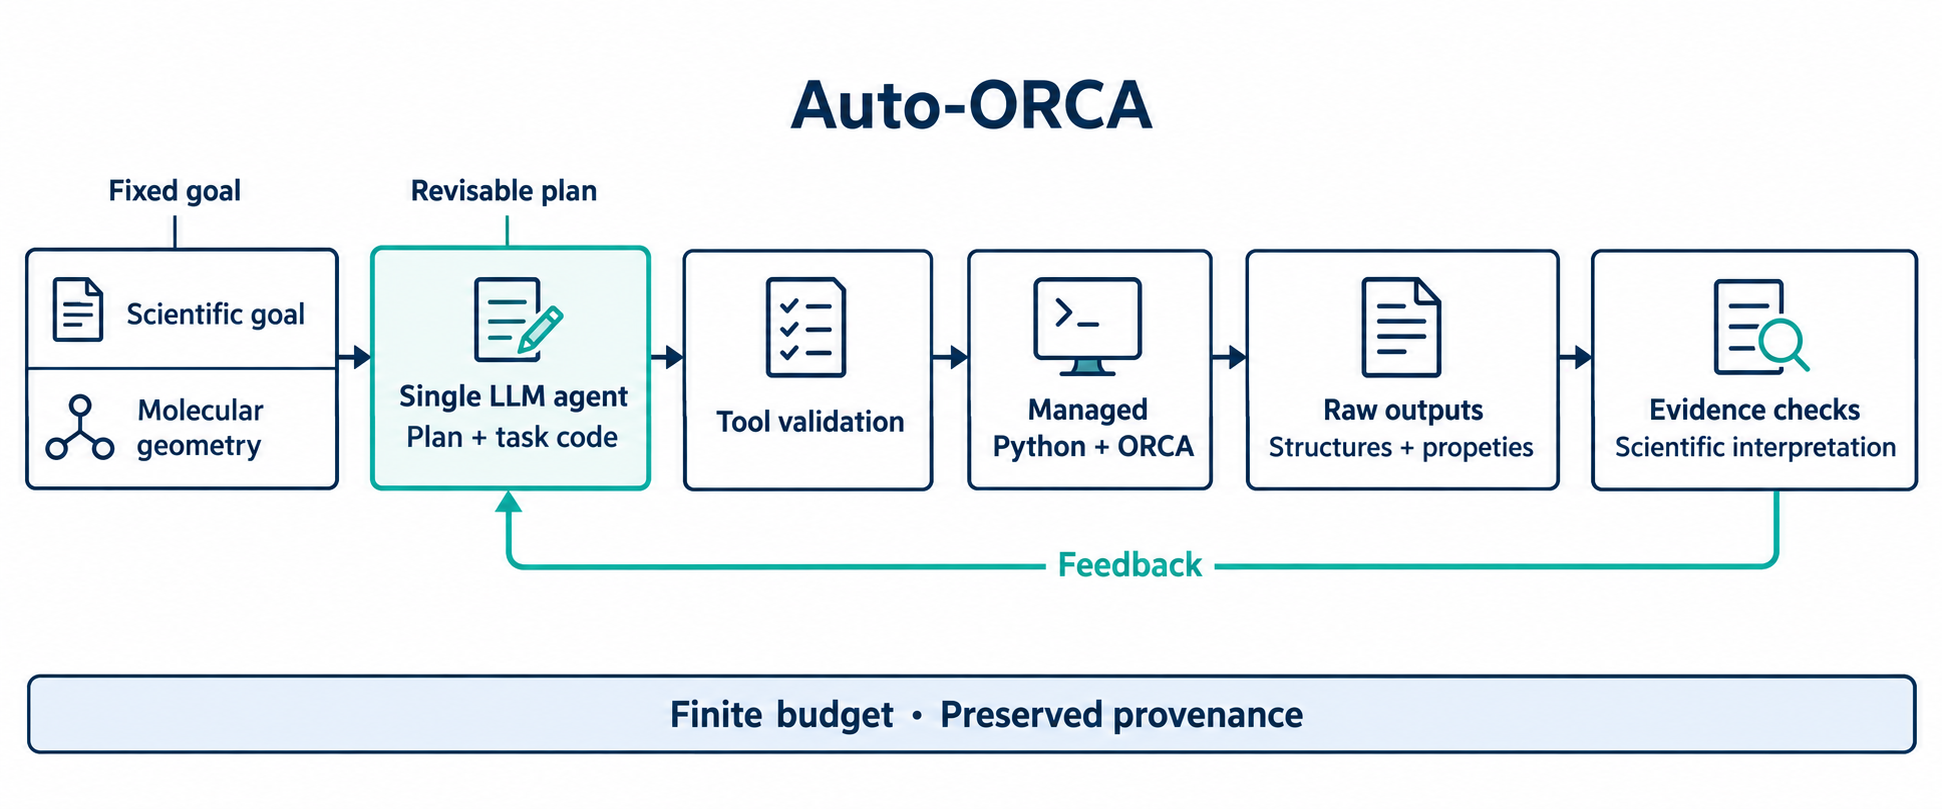
\includegraphics[width=\linewidth]{auto-orca-architecture.png}
  \caption{The single decision loop in Auto-ORCA.
  The original objectives and minimum evidence requirements constrain result evaluation.
  The model uses generic tools to organize managed Python and ORCA execution and revises the plan in response to the returned evidence.}
  \label{fig:architecture}
\end{figure}

Generated code expresses task-specific algorithms; generic tools handle input validation, execution, and artifact management.
For example, a program may construct a finite set of geometries, request an energy calculation for each, and compare the results in consistent units.
OPI input, native ORCA input, and Python calculation requests share one execution entry point~\cite{opi}.
The thin interface returns execution receipts and raw artifacts without embedding an implicit solution algorithm for an individual problem.
The same tools thus support different tasks within explicit execution boundaries.

\subsection{Objective Preservation and Evidence Management}
Request, Plan, Step, Tool, Run, Result, and Artifact represent requirements, computational routes, operations, execution interfaces, run records, results, and raw artifacts, respectively.
Scientific objectives and minimum evidence requirements are stored independently of the Plan; revisions alter only the route to meeting them.

\begin{table}[htbp]
  \centering\small
  \caption{Core representations in Auto-ORCA and their roles in scientific tasks.}
  \label{tab:domain-objects}
  \begin{tabularx}{\linewidth}{>{\raggedright\arraybackslash}p{1.65cm}YY}
    \toprule
    Object & Stored information & Contribution to task reliability\\
    \midrule
    Request & Scientific system, target quantities, conditions, and minimum evidence & Preserves the problem definition and prevents plan revisions from substituting different objectives\\
    Plan & Operation dependencies and the route to the required evidence & Adapts subsequent work to new evidence\\
    Step & Parameters, inputs, and code references for an operation & Defines the scope of the action to be executed\\
    Tool & Interface, execution effects, validation, and output declarations & Converts model intentions into checked operations\\
    Run & Configuration, execution history, and cumulative resource use & Preserves the same cost limits across recovery and retries\\
    Result & Execution facts, checks, observations, and objective evaluation & Distinguishes calculation completion from the scientific meaning of the result\\
    Artifact & Geometries, inputs, programs, and raw outputs & Makes conclusions traceable to specific sources\\
    \bottomrule
  \end{tabularx}
\end{table}

These representations connect scientific meaning to execution.
Explicit user requirements, defaults, inherited conditions, and automatic choices are recorded separately.
References to structures or numerical values bind to specific artifacts and provenance, rather than to a changing ``latest file.''
Different objectives for the same molecule may require different environments or electronic states; conditions are therefore checked per objective rather than unconditionally merged.

The model proposes actions and repairs, whereas the software determines whether an action is executable and whether its outputs satisfy the prescribed checks.
Initial geometries, inputs, generated programs, and each attempt's raw outputs are stored separately, with provenance bound through content verification.
Reading evidence does not implicitly initiate calculations or conversions; additional analyses require explicit operations.
Properties outside standard checks may be retained as observations with provenance, units, and limitations, but neither the model nor task scripts can independently confer scientific validity.

\subsection{Versioned Knowledge Base and On-Demand Retrieval}
\label{sec:knowledge-layer}
Domain knowledge queries within the same agent loop provide traceable references for planning, input preparation, and interpretation.
Sources include the official ORCA 6.1 manual~\cite{orcamanual}, OPI 2.0 documentation~\cite{opi}, RDKit 2025.09.6 documentation, and project-maintained guides on input preparation, method selection, and output diagnosis.
Table~\ref{tab:knowledge-sources} summarizes their roles.

\begin{table}[H]
  \centering\small
  \caption{Knowledge sources used by Auto-ORCA and their roles in autonomous calculations.}
  \label{tab:knowledge-sources}
  \begin{tabularx}{\linewidth}{>{\raggedright\arraybackslash}p{2.8cm}YY}
    \toprule
    Source & Main content & Supported decisions\\
    \midrule
    Official ORCA manual & Input structure, methods and basis sets, optimization, frequencies, and properties & Preparing inputs, verifying options, and identifying diagnostic references\\
    OPI and RDKit documentation & Version-specific interfaces and structure-processing procedures & Preparing structures, writing Python task code, and connecting to calculation interfaces\\
    Project task guides & Principles of input preparation, method selection, and output diagnosis & Preserving conditions, organizing execution dependencies, and identifying repair directions\\
    \bottomrule
  \end{tabularx}
\end{table}

The agent retrieves relevant passages and archives their documents, versions, source locations, and verification metadata.
Retrieval supports planning, input preparation, diagnosis, and repair as needed.
Computational conclusions remain grounded in actual ORCA outputs and corresponding checks.

\subsection{Unified Execution and Observations of Additional Properties}
Although the model can generate task algorithms, execution responsibilities must remain centralized.
Tool definitions specify parameter constraints, execution effects, and outputs; OPI, native input, and internal calculation requests follow the same management procedures.
A program may combine several calculations to address a scientific question, but each retains its own input, geometry, execution facts, and artifacts.
Changing the input representation does not alter resource limits or minimum evidence requirements.

Result acquisition involves distinct evidence levels.
A readable raw file establishes that evidence is accessible; successful field extraction establishes that a particular datum has been obtained; only the corresponding output checks support interpretation within their defined scope.
For properties outside existing checks, generated code may extract and organize observations with provenance, enabling reportable analyses while retaining their validation status.
This expands task expressibility without treating a script's ``pass'' assertion or normal exit code as a scientific judgment.

For example, tensor-analysis code may read a matrix from raw output and calculate its trace, but reliable interpretation also depends on correct atom indices, coordinate directions, and units.
Similarly, scan code may request calculations at several angles, but a target-angle label alone does not demonstrate that the final geometry satisfies the constraint.
The model proposes the analysis; execution and verifiable evidence delimit its conclusions.

\subsection{Feedback, Resources, and Termination}
Feedback preserves original objectives, current results, applicable diagnostics, and queryable evidence sources.
Error diagnostics help locate input, program, or numerical-solution failures; successful outputs help determine whether additional geometry checks, sampling, or cross-result analyses are required.
Uncertain execution states require reconciliation of existing facts before further action to avoid duplicate launches.

Resource constraints cover generated programs and their internal ORCA calculations.
Let $B_k$ be the limit for budget dimension $k$, $U_k$ the cumulative usage, and $r_k$ the reservation for a new action.
Execution requires
\begin{equation}
  U_k+r_k\leq B_k.
\end{equation}
Internal calculations, code retries, and model-based corrections count toward cumulative usage; pausing or resuming does not reset consumption.
Generated code accesses input copies, necessary runtime libraries, and task artifact directories only within a managed task environment.
Completed results and unanswered questions are retained after termination.

Repairs must preserve original objectives and still-valid evidence.
Input-format corrections, code repairs, and scientific-method adjustments have different implications and should be identified separately in subsequent actions.
Failure does not invalidate other completed calculations, nor does success automatically validate unresolved matters.
Unclear execution provenance requires reconciliation of existing processes and artifacts before repetition.

Feedback informs subsequent actions within the limits of original scientific conditions, actual evidence, and remaining resources.

\subsection{Comparison of Open-Loop and Closed-Loop Mechanisms}
We distinguish open-loop planning from closed-loop execution~\cite{autodft} to clarify result feedback (Figure~\ref{fig:open-closed-loop}).
In open-loop operation, the model specifies a complete route initially, and execution primarily follows predetermined steps and rules.
It may include error detection, rule-based retries, and routine recovery.
Closed-loop operation returns new scientific evidence to model decision-making, allowing unexecuted steps to change as understanding develops.

\begin{figure}[htbp]
  \centering
  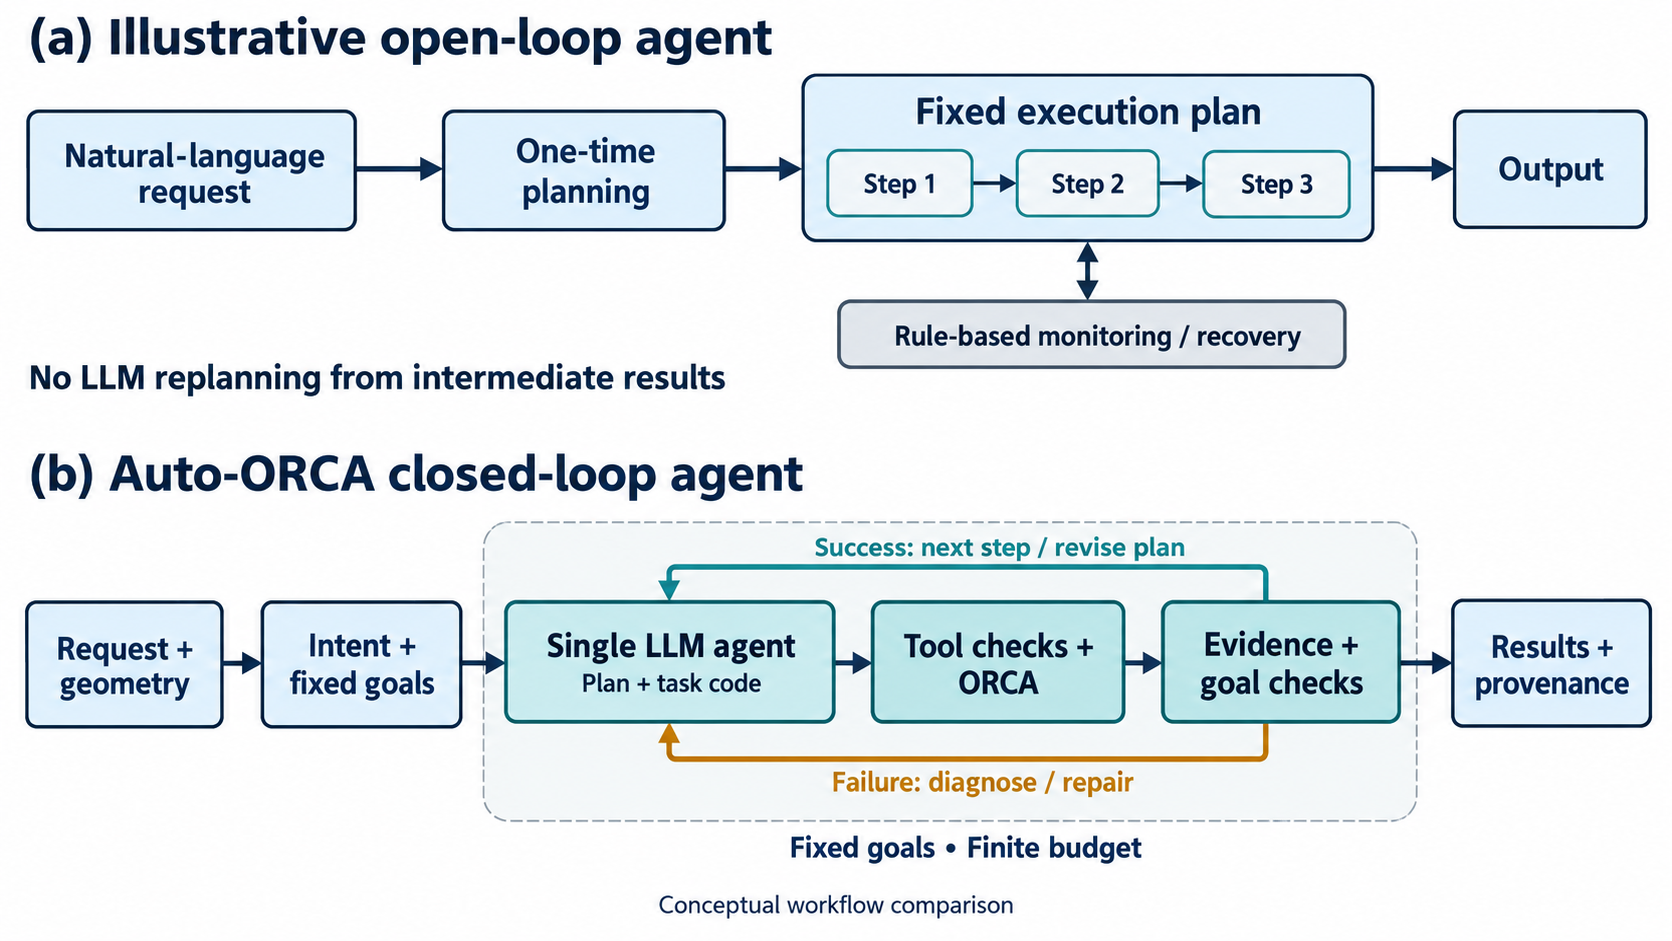
\includegraphics[width=\linewidth]{open-loop-vs-auto-orca.png}
  \caption{Comparison of the mechanisms underlying an open-loop agent and the Auto-ORCA closed-loop workflow.}
  \label{fig:open-closed-loop}
\end{figure}

In molecular calculations, later steps often require information available only after earlier steps have been completed.
For example, frequency analysis must be tied to the optimized structure actually obtained; conformer comparison requires identification of candidates with usable energies; and environmental comparisons require verification that the two calculations share a common geometry.
Returning this information to the decision process after execution allows plans to be grounded in evidence already obtained.
The Auto-ORCA closed loop thus supports exception handling and scientific progress through successful results.

\begin{table}[htbp]
  \centering\small
  \caption{Mechanistic comparison of open-loop operation and Auto-ORCA.}
  \label{tab:loop-comparison}
  \begin{tabularx}{\linewidth}{>{\raggedright\arraybackslash}p{2.35cm}YY}
    \toprule
    Dimension & Illustrative open-loop agent & Auto-ORCA closed-loop organization\\
    \midrule
    Planning & Specifies the complete sequence and main parameters at the outset & Establishes an initial route and determines subsequent actions using new evidence\\
    Successful results & Supply inputs to predetermined steps and predefined post-processing & Also inform objective progress and the suitability of subsequent actions\\
    Exception handling & Monitors, retries, or stops according to predefined rules & Proposes checked repairs using diagnostics, previous attempts, and objectives\\
    Algorithm expression & Executes operations specified in the initial plan & Generates bounded task code for the problem and combines generic tools\\
    Condition preservation & Relies on the initial plan and execution rules & Stores original objectives independently and rechecks conditions after plan revisions\\
    Final delivery & Summarizes outputs from the executed route & Links results, actual conditions, provenance, and unresolved issues to each objective\\
    \bottomrule
  \end{tabularx}
\end{table}

Auto-ORCA explicitly connects decision-making and execution responsibilities.
A single agent continually addresses the same scientific objectives, generic tools implement actions, and raw artifacts inform subsequent decisions.
Computational, analytical, and interpretive requirements share a task without requiring a separate complete workflow for every combination.
Adaptable routes and stable problem definitions provide a basis for extending to more complex potential-energy-surface exploration.

\section{End-to-End Workflow from Natural Language to a Computational Report}
\label{sec:end-to-end-workflow}
Auto-ORCA transforms scientific questions into executable tasks with explicit inputs, conditions, and evidence sources.
One agent loop coordinates natural-language input, intent recognition and condition confirmation, objective specification, planning with knowledge retrieval as needed, task code generation, ORCA execution, result checking and feedback, and final delivery.
Subsequent actions depend on established facts and may include evidence queries, plan revisions, and supplementary analyses.
The following subsections trace this information flow.

\subsection{Natural-Language Input and Scientific Intent Recognition}
The interface accepts natural-language descriptions and user-provided structures, output files, or existing-result references.
The system preserves the original request and identifies four elements: the scientific system, required physical quantities, computational conditions, and expected deliverables.
For example, ``optimize ethanol and calculate its vibrational frequencies'' must specify the molecule, optimization, frequencies at the optimized structure, and delivery of corresponding coordinates and numerical results.
``Compare the energies of the same structure in two environments'' additionally requires preservation of the common geometry and calculation pairing.

Intent recognition produces a checkable structured candidate recording the system, objectives, geometric relationships, conditions, minimum evidence, and unresolved information.
Key fields retain their supporting source text.
The software checks the candidate against the user message before storing normalized requirements.
This helps preserve qualifiers such as ``the same geometry,'' ``the first five states,'' and ``the complete tensor,'' reducing the risk of recognizing only broad task categories while omitting delivery requirements.

\subsection{Condition Clarification and Objective Specification}
The method, basis set, charge, multiplicity, environment, and geometry source define the computational problem.
The system distinguishes explicit user conditions, traceable inherited conditions, defaults, and authorized automatic choices.
Missing information remains unresolved; the agent may ask targeted questions when omissions affect the system or result meaning.
For delegated method or basis-set selection, the system may record a justified choice and check compatibility with remaining conditions before launch.

After condition confirmation, objectives and minimum evidence requirements are stored independently of the execution plan.
A request may contain multiple objectives, each with its own constraints on the system, environment, electronic state, and geometric relationships.
For example, gas-phase and solution energy comparisons must preserve two environment-specific objectives and their common geometry, rather than an undifferentiated ``energy'' field.
Fixed objectives allow flexible routes: plans may add parsing steps or repair inputs but must address the original question.

\subsection{On-Demand Knowledge Queries to Support Operations}
\label{sec:knowledge-retrieval}
When an operation requires information on software syntax, methods, or property definitions, the agent formulates a specific query.
It selects sources, formulates search terms, retrieves matching passages, and assesses their support for the decision.
For example, frequency tasks may require optimization and vibrational-analysis documentation; Python task code may require version-specific OPI interface documentation; and input diagnosis may use ORCA logs to locate relevant manual sections.

Knowledge queries may also support result interpretation.
References can clarify physical quantities, such as the relationship between nuclear magnetic shielding and chemical shifts or the distinction between electronic energy differences and free energies.
Numerical values, geometries, and convergence states are read from corresponding raw artifacts.
The final report can thus state the operational rationale, actual conditions, and numerical sources.

\subsection{Organizing the Computational Plan by Dependencies}
The agent translates objectives into interdependent operations: reading or preparing structures, generating inputs, executing calculations, extracting properties, and organizing results.
Each step identifies its system, registered input files, tool, and expected outputs.
The software checks objective alignment, file dependencies, tool permissions, and available budgets.
Execution requires available prerequisite data that satisfy the step's checks.

The plan expresses scientific ordering as data dependencies.
Post-optimization frequencies require the corresponding final structure; energy rankings preserve energy--candidate associations; and rotational consistency analysis requires results for two orientations and the rotation definition.
Route changes create a new plan version while preserving executed inputs and attempt records.
Exploration can thus adapt while retaining each result's computational route.

\subsection{Task Code Generation through a Unified Tool Boundary}
For tasks difficult to express through fixed interfaces, the agent may write Python task code and native ORCA input for repeated calculations, field extraction, matrix organization, or deterministic derived-quantity analysis.
Code is stored with provenance before an execution step references it.
Execution requires checks of code and input identities, file dependencies, and task declarations.
Generated programs run in a managed environment; internal ORCA requests use the unified entry point.

With this organization, new tasks are expressed primarily through changes in operation composition and task programs.
Conformer comparison manages geometries and energies; excited-state analysis organizes state-resolved outputs; shielding analysis preserves atom indices and matrix components.
All three share file-writing, execution, querying, and archiving mechanisms.
Programs provide computational capabilities, while the tool boundary preserves traceability of actual inputs, resource consumption, and raw artifacts.

\subsection{Execution, Monitoring, and Raw Artifact Archiving}
Before launch, the system verifies actual inputs, geometry, conditions, permissions, and remaining resources, and records the operation separately.
Task code and its internal ORCA calculations share a controlled execution environment and cumulative resource constraints.
Launch is confirmed by a trusted execution receipt.
Uncertain execution states require reconciliation of existing processes and receipts before they can be treated as unstarted, preventing duplicate calculations.

After execution, inputs, standard output, error logs, structure files, and property files are archived and linked to results.
Records are preserved for both normal completion and failure.
These records support diagnosis and feedback from both numerical results and failure causes.

\subsection{Result Checking and Evidence-Based Continuation}
The main loop reevaluates objectives after each new result, before choosing the next action.
Checks cover the actual conditions, file integrity, output readability, and applicable scientific validation.
Existing checks govern covered outputs; task code may extract new properties as observations with provenance, units, and validation statements.
Successful reading, calculation completion, reportable observations, and verified scientific requirements are recorded separately to ground conclusions in actual evidence.

Successful feedback may initiate necessary analysis.
Completed optimization requires acquisition of the final structure and frequency evidence; completed candidate calculations require consolidated associations and consistent energy units.
Failure feedback identifies fields, program errors, or ORCA log locations for targeted repairs and, when needed, focused documentation queries to inform revisions.
Repairs use new inputs or subsequent steps, preserving original objectives and still-valid sources; original failures remain accessible.

The system checks for remaining executable work toward current objectives.
If approved subsequent steps, recoverable failures, or analyses of archived originals remain available, feedback identifies continuation options that the final delivery check uses to prevent premature termination.
Existing files may support continuation through parsing alone, directing further effort toward actual evidence gaps.

\subsection{Final Output and Verifiable Delivery}
When the task reaches a deliverable state, or when resources, permissions, or specific execution conditions require termination, the system consolidates the correspondence between objectives and evidence.
Final outputs include the question, actual methods, numerical results or structures, necessary units and reference definitions, calculation and validation status, artifact locations, and outstanding work.
Method-selection rationales refer directly to saved records, while numerical values are traced to the corresponding raw outputs and analytical sources.
Retrieval records link knowledge sources to document versions and passage locations, preserving traceability of both the operational rationale and the result sources.

Tables facilitate comparison, raw files support verification, and limitations indicate what additional evidence is needed.
The reported calculation success rate describes whether ORCA calculations for the seven questions completed normally and produced numerical results.
Each result's scientific conclusions remain separately delimited by its method, geometry, and property evidence.

\subsection{Illustration: Information Flow in Ethanol Optimization and Frequency Analysis}
The table below traces the information flow from a natural-language request to final delivery for ethanol optimization and vibrational frequency analysis.

\begin{table}[htbp]
  \centering\small
  \caption{Progressive specification of information in the ethanol task.
  The illustrative natural-language input is ``Optimize neutral singlet ethanol in the gas phase using r$^{2}$SCAN-3c and report its vibrational frequencies.''}
  \label{tab:workflow-example}
  \begin{tabularx}{\linewidth}{>{\raggedright\arraybackslash}p{2.35cm}YY}
    \toprule
    Stage & Information established & Information passed to the next stage\\
    \midrule
    Intent recognition & Ethanol; structure optimization; vibrational frequencies & Two types of results and the requirement to calculate frequencies at the optimized structure\\
    Condition confirmation & Gas phase, neutral singlet, r$^{2}$SCAN-3c & Confirmed method, built-in basis set, and geometry source\\
    On-demand knowledge queries & Relevant references on the method, interface, or frequency settings & Citable source passages, software versions, and operational rationale\\
    Planning & Structure preparation, calculation, extraction, and interpretation & Inputs and required outputs for each operation\\
    Code and input & Actual ORCA input and any required analysis programs & File identities, conditions, and resource declarations\\
    Execution and archiving & Raw outputs, final coordinates, and property files & Actual completion status and readable artifacts\\
    Checking and analysis & Convergence records, mode count, and imaginary frequencies & Evidence concerning energy, frequencies, and local stability\\
    Result delivery & Methods, numerical values, coordinates, and interpretation & Readable conclusions and computational materials available for further use\\
    \bottomrule
  \end{tabularx}
\end{table}
\section{Computational Methods and Agent Capability Assessment}
\subsection{Computational Settings and Scientific Tasks}
Calculations were performed using ORCA 6.1.1 and organized through OPI 2.0.0 and the unified execution interface.
The local resource allocation comprised four CPU cores, a memory limit of 1024 MiB for the computational process tree,
and an ORCA MaxCore setting of 192 MiB per process.
MaxCore is an internal ORCA memory parameter and was configured separately from the total memory limit on the process tree.

Table~\ref{tab:task-overview} lists the methods actually used for the seven test problems.
All systems for which calculations were completed were neutral singlets.
The r$^{2}$SCAN-3c calculations used the built-in def2-mTZVPP basis set~\cite{r2scan3c};
other methods and basis sets are reported individually according to the calculations performed,
with the basis sets following the def2 definitions~\cite{def2}.
Vertical excitations were calculated using full linear-response TDDFT~\cite{tddft},
and the aqueous environment was represented by the CPCM continuum model~\cite{cpcm}.
Except for the explicitly identified geometry optimizations and constrained optimizations,
all results correspond to specified fixed geometries.

\subsection{Design of the Agent Capability Assessment}
\label{sec:agent-evaluation-design}
The seven problems assess \textbf{the ability of the Auto-ORCA agent to translate scientific requests
into actual calculations and interpretable results}.
The assessment spans task interpretation, preservation of conditions, input preparation, and result organization.
The selected molecules and properties require structure preparation before property calculation,
finite candidate management, comparable conditions, organization of multiple excited states, or tensor analysis.
The checks examine whether the agent initiates and completes actual ORCA calculations
and clearly reports the calculated system, conditions, and scope of the conclusions.

T1--T3 address local structure determination, comparison of candidate geometries,
and constrained calculations along an internal coordinate, respectively---common components of potential energy surface exploration.
T4, T5, H1, and H2 extend the assessment to excited states, environmental changes, and response tensors,
testing whether the same execution interface supports different output forms.
Task identifiers only associate problems with results; capability assessments use actual inputs, outputs, and geometry records.
Table~\ref{tab:agent-capability-design} specifies the targeted capabilities and required evidence.

\begin{figure}[htbp]
  \centering
  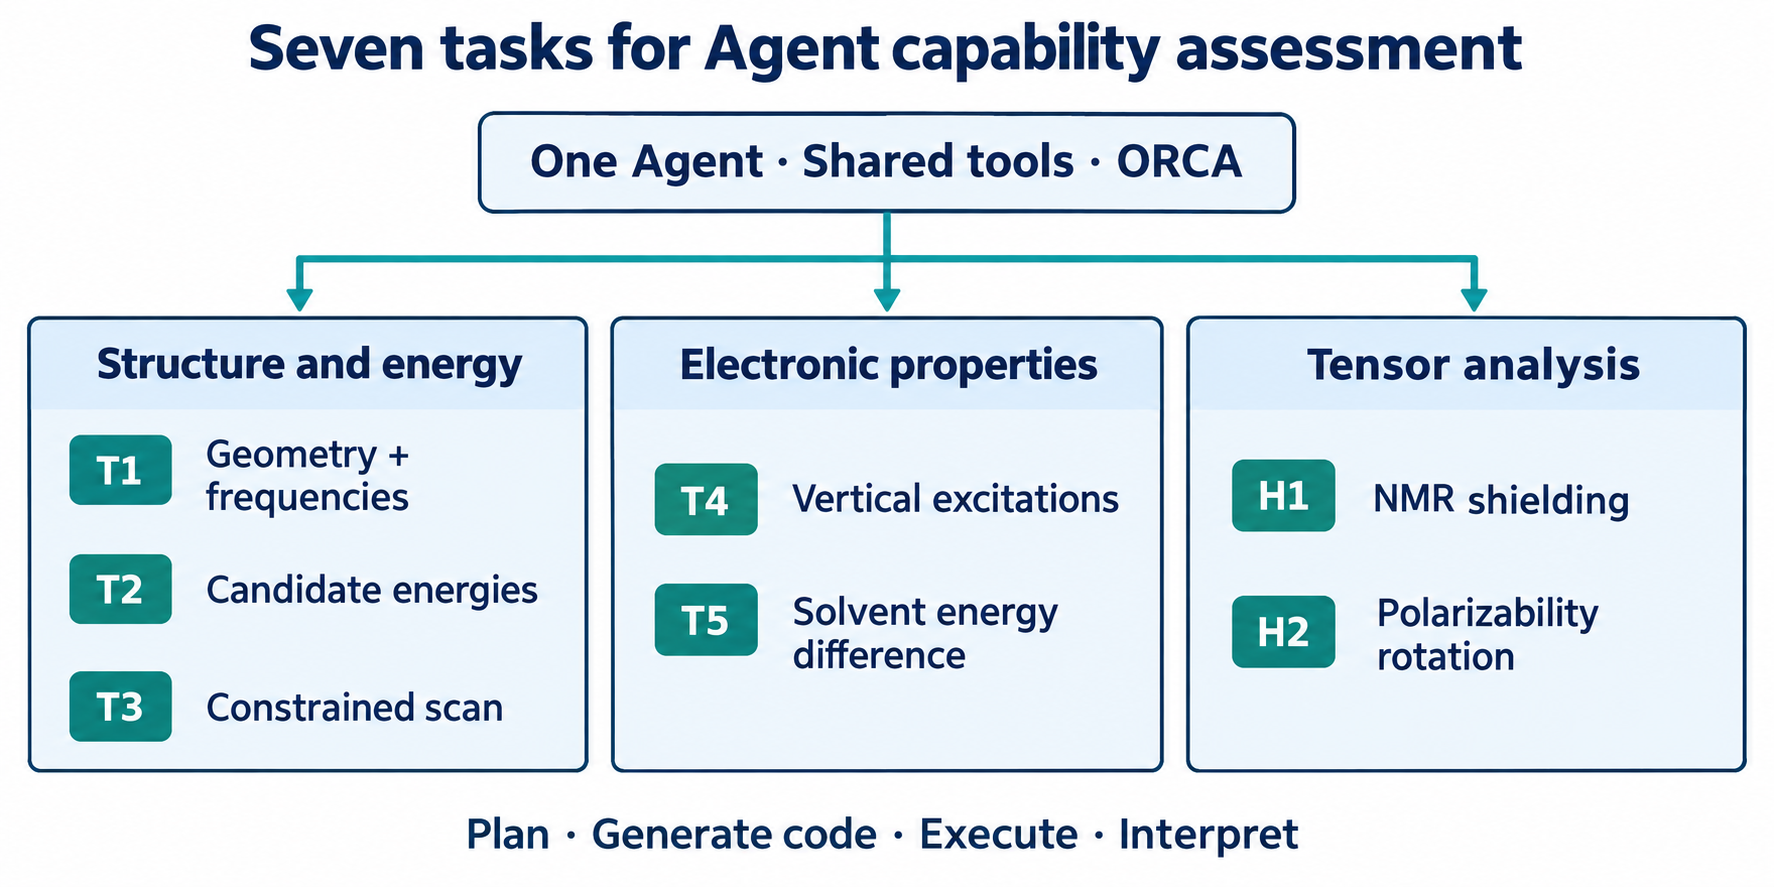
\includegraphics[width=\linewidth]{agent-capability-map.png}
  \caption{Scope of the agent capability assessment across seven problems.
  All problems use the same task organization and ORCA execution mechanism,
  while examining distinct operational requirements for structures and energies, electronic properties, and tensor analysis.
  The diagram illustrates the assessment design; the extent of completion is determined by the actual results.}
  \label{fig:agent-capability-map}
\end{figure}

\begin{table}[htbp]
  \centering\small
  \caption{Design of the agent capability assessment.
  The table lists the intended assessment dimensions; the extent of completion is reported with the individual results.}
  \label{tab:agent-capability-design}
  \begin{tabularx}{\linewidth}{lYY}
    \toprule
    Task & Principal capability & Evidence to examine\\
    \midrule
    T1 & Organize optimization--frequency dependencies and preserve structural provenance
       & Optimization convergence, final geometry, frequency count, and imaginary frequencies\\
    T2 & Organize a finite set of candidate calculations, associate identifiers, and standardize energy units
       & Candidate geometries, individual energies, reference candidate, and unit conversions\\
    T3 & Generate a loop for constrained calculations and maintain correspondence between target inputs and actual geometries
       & Constraint inputs, outputs at each point, final dihedral angles, and incomplete points\\
    T4 & Configure native property calculations and associate outputs across excited states
       & Method and TDA settings, convergence records, state-resolved energies, and oscillator strengths\\
    T5 & Preserve comparable geometries and methods when changing the environment
       & Geometries in both environments, basis and solvent settings, and the sign of the energy difference\\
    H1 & Parse atom-resolved tensors while preserving units and component ordering
       & Atom indices, complete shielding matrices, isotropic values, and units of ppm\\
    H2 & Organize calculations before and after rotation and check tensor consistency
       & Both molecular orientations, rotation definition, polarizability tensors, and comparison residuals\\
    \bottomrule
  \end{tabularx}
\end{table}

\FloatBarrier

Results can be examined at three levels: the actual method, geometry, charge, and multiplicity;
normal termination in the raw ORCA output and preservation of the requested values;
and interpretation against the available evidence.
For example, the lowest single-point energy in a finite set does not establish the global minimum conformer,
and an electronic energy difference at fixed geometry is not a free energy.
The first two levels establish computational provenance; the third determines how far the outputs answer the scientific question.

Table~\ref{tab:agent-capability-design} therefore describes assessment coverage, not uniformly demonstrated capabilities.
The completed calculations illustrate diverse task formulations, execution, and numerical delivery,
but dependencies, geometric correspondence, and property interpretation still require individual verification.
Without repeated trials or comparison systems, the seven-problem success rate cannot estimate success on unseen tasks.
Repeating the problems under identical goals and conditions can resolve verification gaps
and distinguish computational completion, verifiability of results, and fulfillment of scientific goals.

\subsection{Calculation Success Rate and Interpretation of Results}
Normal-termination records in the raw ORCA output serve as evidence that a calculation has completed.
Each problem in this study is classified as \textbf{successful} if a corresponding ORCA calculation has terminated normally
and its numerical results have been retained; a problem with no actual numerical result is classified as \textbf{incomplete}.
This classification includes the six completed points in T3 despite the uncomputed endpoint and the limitations of angle verification.
\begin{equation}
  R_{\mathrm{calc}}=\frac{N_{\mathrm{success}}}{N_{\mathrm{questions}}}
  =\frac{6}{7}\approx85.7\%.
  \label{eq:success-rate}
\end{equation}
Each of the seven problems is counted once.
Scientific conclusions depend separately on convergence, geometry, method, and property evidence.
Normal termination alone does not establish a global minimum conformer, a correct torsional barrier,
or a response property directly comparable with experiment.

Relative electronic energies are referenced to a specified member of the candidate set.
Energy conversions use $1\,\Eh=2625.4996394799$ kJ mol$^{-1}$.
Electronic energies, vibrational frequencies, excitation energies, and shielding tensors retain the original output or verification precision.
Raw data and provenance records support inspection and reuse~\cite{fair}.
The reported success rate describes existing results, not the probability of success on arbitrary new tasks;
energy differences without independent references are not used to assess methodological accuracy.

\subsection{Scope of the Evaluation}
The calculation success rate across the seven problems indicates whether the agent has produced actual computational results for those problems.
Assessing numerical accuracy additionally requires confirmation that each calculated value and its independent reference
refer to the same system, geometry, physical quantity, and theoretical conditions.
For tasks with reliable reference values, the coverage of valid matches and the error over the matched subset can be reported separately:
\begin{equation}
  \mathrm{Coverage}=\frac{N_{\mathrm{matched}}}{N_{\mathrm{target}}},
  \qquad
  \mathrm{MAE}_{\mathrm{matched}}=
  \frac{1}{N_{\mathrm{matched}}}\sum_{i\in\mathcal M}|y_i-y_i^{\mathrm{ref}}|.
  \label{eq:coverage-accuracy}
\end{equation}
Here, $\mathcal M$ contains only targets with established correspondence,
and $y_i$ and $y_i^{\mathrm{ref}}$ use the same units.
If $N_{\mathrm{matched}}=0$, the error is not evaluable.
This formulation defines conditions for future accuracy comparisons.
Without independent high-accuracy references, this study reports no empirical MAE
and does not treat energy differences between methods or geometries as numerical errors.

\section{Results of the Agent Capability Assessment}
\subsection{Overview of the Seven Test Cases}
The following seven scientific questions were used to evaluate the task organization and execution capabilities of Auto-ORCA Agent;
their intended capability coverage is summarized in Table~\ref{tab:agent-capability-design}.
Table~\ref{tab:task-overview} summarizes the methods actually used and the results obtained for each case.
T1--T5 and H1 were classified as successful calculations, whereas H2 remained incomplete, yielding a calculation success rate of $6/7=85.7\%$.
The numerical results and their scientific interpretation are presented below.

\begin{table}[H]
  \centering\small
  \caption{Methods actually used and results obtained for the seven test cases.
  Success indicates that an ORCA calculation terminated normally and produced the corresponding numerical results.
  }
  \label{tab:task-overview}
  \begin{tabularx}{\linewidth}{l>{\raggedright\arraybackslash}p{2.6cm}>{\raggedright\arraybackslash}p{3.1cm}>{\raggedright\arraybackslash}p{1.8cm}Y}
    \toprule
    ID & Question & Actual method & Status & Principal results\\
    \midrule
    T1 & Ethanol optimization and frequencies & r$^{2}$SCAN-3c & Success & Converged optimization; 21 positive frequencies and no imaginary frequencies\\
    T2 & Candidate energies for \textit{n}-hexane & r$^{2}$SCAN-3c single-point calculations & Success & Energy ranking of six candidate geometries\\
    T3 & Dihedral scan of \textit{n}-butane & r$^{2}$SCAN-3c constrained optimization & Success & Six converged points; actual angles remain unverified\\
    T4 & Vertical excitations of acetone & PBE0/def2-SVP, LR-TDDFT & Success & Five singlet excitation energies and oscillator strengths\\
    T5 & Environmental energy differences for ethanol & B3LYP/def2-TZVP and def2-SVP & Success & Gas-phase--CPCM water electronic energy differences with two basis sets\\
    H1 & Nuclear magnetic shielding of HCN & PBE0/def2-TZVP, GIAO & Success & Full shielding tensors for the C, N, and H nuclei\\
    H2 & Formaldehyde polarizability and rotational consistency & No actual calculation results & Incomplete & No polarizability values obtained\\
    \bottomrule
  \end{tabularx}
\end{table}

\subsection{T1: Geometry Optimization and Vibrational Frequencies of Ethanol}
\paragraph{Question}
Optimize the geometry of ethanol and use its vibrational frequencies to assess whether the resulting structure is a local minimum.

\paragraph{Method}
Geometry optimization and vibrational frequency calculations were performed using r$^{2}$SCAN-3c with its built-in def2-mTZVPP basis set for a neutral singlet in the gas phase.

\paragraph{Results}
\textbf{Successful calculation.} The geometry optimization converged, giving an optimized electronic energy of $-155.002345492244\,\Eh$.
The calculation yielded 21 positive vibrational frequencies, six zero-frequency translational and rotational modes after projection, and no imaginary frequencies.
All positive frequencies are listed in Table~\ref{tab:t1-frequencies}.
These results support assignment of the structure as a local minimum at the employed level of theory; they do not establish that it is the global minimum-energy conformer.
The optimized coordinates are retained in the XYZ file associated with the corresponding ORCA output.

\begin{table}[H]
  \centering\small
  \caption{The 21 positive vibrational frequencies of ethanol, in cm$^{-1}$.}
  \label{tab:t1-frequencies}
  \begin{tabular}{rrrrrrr}
    \toprule
    270.90 & 298.95 & 425.86 & 811.51 & 882.13 & 1052.13 & 1066.45\\
    1134.41 & 1282.25 & 1371.13 & 1396.18 & 1418.25 & 1483.33 & 1487.57\\
    1509.53 & 2969.59 & 3004.65 & 3061.83 & 3088.36 & 3105.66 & 3819.31\\
    \bottomrule
  \end{tabular}
\end{table}

\subsection{T2: Single-Point Electronic Energies of Candidate \textit{n}-Hexane Conformers}
\paragraph{Question}
Compare the electronic energies of candidate \textit{n}-hexane geometries and determine their relative energy ordering within the calculated set.

\paragraph{Method}
Single-point calculations were performed separately for six stored candidate geometries using r$^{2}$SCAN-3c for neutral singlets in the gas phase.
Relative energies were referenced to cand\_05.

\paragraph{Results}
\textbf{Successful calculation.} Electronic energies were obtained for all six candidates, as reported in Table~\ref{tab:t2-energies}.
Within this set, cand\_05 had the lowest energy, whereas cand\_03 was higher by 12.608656~kJ~mol$^{-1}$.
These are single-point results for candidate geometries; they do not demonstrate that all six conformers underwent DFT optimization,
nor do they establish the global minimum-energy conformer or a free-energy ordering.

\begin{table}[H]
  \centering\small
  \caption{Single-point electronic energies of six candidate \textit{n}-hexane geometries.}
  \label{tab:t2-energies}
  \begin{tabular}{lrr}
    \toprule
    Candidate & Electronic energy / $\Eh$ & Relative energy / kJ mol$^{-1}$\\
    \midrule
    cand\_05 & $-236.992066202851$ & 0.000000\\
    cand\_04 & $-236.991445556657$ & 1.629506\\
    cand\_01 & $-236.991444090308$ & 1.633356\\
    cand\_00 & $-236.991421448668$ & 1.692802\\
    cand\_06 & $-236.991245997872$ & 2.153448\\
    cand\_03 & $-236.987263819406$ & 12.608656\\
    \bottomrule
  \end{tabular}
\end{table}

\subsection{T3: Dihedral Scan of \textit{n}-Butane}
\paragraph{Question}
Obtain the electronic energies of \textit{n}-butane at different target dihedral angles through constrained optimization and examine the variation in torsional potential energy.

\paragraph{Method}
The main calculations employed r$^{2}$SCAN-3c for a neutral singlet in the gas phase, with constrained optimization at specified target dihedral angles.
An additional B3LYP/def2-TZVP calculation point is reported separately, together with the result of its geometry verification.

\paragraph{Results}
\textbf{Successful calculation.} Normal ORCA termination and optimization convergence were recorded for all six r$^{2}$SCAN-3c calculation points;
the results are given in Table~\ref{tab:t3-energies}.
The first column contains only the target-angle labels specified in the inputs.
The actual angles reported by the generated script conflict with these input labels and have not yet been confirmed through independent geometry verification.
Consequently, the energies are genuine computational outputs, but the labels cannot be treated as verified actual dihedral angles or used to establish a torsional barrier.
In particular, the high energy associated with the $+120^\circ$ label cannot be directly interpreted as a reliable physical barrier.

\begin{table}[H]
  \centering\small
  \caption{Six constrained optimization points for \textit{n}-butane.
  Angles denote input target labels; relative energies are the stored numerical values.
  }
  \label{tab:t3-energies}
  \begin{tabular}{rrr}
    \toprule
    Input target angle / $^\circ$ & Electronic energy / $\Eh$ & Relative energy / kJ mol$^{-1}$\\
    \midrule
    $-180$ & $-158.392470368263$ & 0.000000\\
    $-120$ & $-158.387146187943$ & 13.978634\\
    $-60$ & $-158.391526560891$ & 2.477966\\
    $0$ & $-158.383528626170$ & 23.476541\\
    $+60$ & $-158.391526702130$ & 2.477595\\
    $+120$ & $-158.358972460497$ & 87.948745\\
    \bottomrule
  \end{tabular}
\end{table}

The input target angle for the B3LYP/def2-TZVP calculation point was $-180^\circ$.
Independent geometry verification gave an actual angle of $179.999995786^\circ$, consistent with the target under angular periodicity;
the converged electronic energy was $-158.397118300397\,\Eh$.
Because this point was obtained using a different method, it is excluded from the relative energies in Table~\ref{tab:t3-energies}.

\subsection{T4: The First Five Singlet Vertical Excitations of Acetone}
\paragraph{Question}
Obtain the excitation energies, wavelengths, and oscillator strengths of the first five singlet vertical excitations of acetone.

\paragraph{Method}
Five singlet excited states were calculated at a fixed, prepared geometry using PBE0/def2-SVP for a neutral singlet in the gas phase,
with full linear-response TDDFT (LR-TDDFT; \code{TDA=false}).
Oscillator strengths were taken from the length-gauge output of ORCA.

\paragraph{Results}
\textbf{Successful calculation.} Convergence was recorded for both the SCF and response calculations; numerical results for the five excited states are listed in Table~\ref{tab:t4-excitations}.
The lowest singlet vertical excitation energy was 4.197061~eV, corresponding to a wavelength of 295.4~nm.

\begin{table}[H]
  \centering\small
  \caption{The first five singlet vertical excitations of acetone.
  Oscillator strengths $f$ are dimensionless.
  }
  \label{tab:t4-excitations}
  \begin{tabular}{crrr}
    \toprule
    Excited state & Excitation energy / eV & Wavelength / nm & Oscillator strength $f$\\
    \midrule
    $S_{1}$ & 4.197061 & 295.4 & 0.000007493\\
    $S_{2}$ & 7.464499 & 166.1 & 0.023781213\\
    $S_{3}$ & 8.406988 & 147.5 & 0.001899769\\
    $S_{4}$ & 8.572306 & 144.6 & 0.060276158\\
    $S_{5}$ & 8.640904 & 143.5 & 0.004121254\\
    \bottomrule
  \end{tabular}
\end{table}

\subsection{T5: Electronic Energy Differences between Gas-Phase Ethanol and Ethanol in CPCM Water}
\paragraph{Question}
Compare the electronic energies of ethanol at the same geometry in the gas phase and in a CPCM water environment.

\paragraph{Method}
Calculations employed B3LYP for a neutral singlet with the def2-TZVP and def2-SVP basis sets, respectively.
For each basis set, the gas-phase and aqueous-environment calculations used the same initial geometry; this geometry was not the optimized structure from T1.
The energy difference was defined as $\Delta E=E_{\mathrm{water}}-E_{\mathrm{gas}}$.

\paragraph{Results}
\textbf{Successful calculation.} Two ORCA calculations, one in the gas phase and one in CPCM water, were completed for each basis set.
Table~\ref{tab:t5-energies} reports the electronic energies, and Table~\ref{tab:t5-differences} reports their differences.
The negative signs indicate that, for the corresponding model and fixed geometry, the electronic energy in the aqueous environment was lower than that in the gas phase.
These quantities are \textbf{electronic energy differences, not hydration free energies}.

\begin{table}[H]
  \centering\small
  \caption{Electronic energies of ethanol in the gas phase and in CPCM water.}
  \label{tab:t5-energies}
  \begin{tabular}{lrr}
    \toprule
    Basis set & Gas-phase electronic energy / $\Eh$ & CPCM water electronic energy / $\Eh$\\
    \midrule
    def2-TZVP & $-155.002778990957$ & $-155.009740144896$\\
    def2-SVP & $-154.817054999208$ & $-154.823380641772$\\
    \bottomrule
  \end{tabular}
\end{table}

\begin{table}[H]
  \centering\small
  \caption{Electronic energy differences for ethanol in water relative to the gas phase.}
  \label{tab:t5-differences}
  \begin{tabular}{lrr}
    \toprule
    Basis set & $\Delta E$ / $\Eh$ & $\Delta E$ / kJ mol$^{-1}$\\
    \midrule
    def2-TZVP & $-0.006961153939$ & $-18.276507$\\
    def2-SVP & $-0.006325642564$ & $-16.607972$\\
    \bottomrule
  \end{tabular}
\end{table}

\subsection{H1: GIAO Nuclear Magnetic Shielding Tensors of HCN}
\paragraph{Question}
Obtain the nuclear magnetic shielding tensor and isotropic shielding of each atom in HCN.

\paragraph{Method}
Calculations were performed at a fixed initial geometry using PBE0/def2-TZVP and the GIAO method for a neutral singlet in the gas phase.
The atom order was C$_0$, N$_1$, and H$_2$.

\paragraph{Results}
\textbf{Successful calculation.} The total electronic energy was $-93.345070922944\,\Eh$.
The isotropic shielding values printed by ORCA are listed in Table~\ref{tab:h1-isotropic}; the full total shielding tensors are given in Eq.~\eqref{eq:h1-tensors}.
The tensor components are expressed in ppm, with both rows and columns ordered as X, Y, and Z; the three decimal places of the original output are retained.

\begin{table}[H]
  \centering\small
  \caption{Isotropic nuclear magnetic shielding values for HCN.}
  \label{tab:h1-isotropic}
  \begin{tabular}{cr}
    \toprule
    Atom & Isotropic shielding / ppm\\
    \midrule
    C$_0$ & 79.051\\
    N$_1$ & $-34.068$\\
    H$_2$ & 29.850\\
    \bottomrule
  \end{tabular}
\end{table}

\begin{equation}
  \begin{aligned}
    \bm{\sigma}_{\mathrm{C}_0}&=\begin{pmatrix}
      279.306 & -0.724 & -0.000 \\
      -1.638 & -21.077 & 0.000 \\
      -0.000 & 0.000 & -21.076
    \end{pmatrix},\\[0.8em]
    \bm{\sigma}_{\mathrm{N}_1}&=\begin{pmatrix}
      340.398 & -1.842 & -0.000 \\
      -0.044 & -221.291 & 0.000 \\
      0.000 & 0.000 & -221.309
    \end{pmatrix},\\[0.8em]
    \bm{\sigma}_{\mathrm{H}_2}&=\begin{pmatrix}
      39.712 & 0.055 & -0.000 \\
      -0.114 & 24.919 & -0.000 \\
      -0.000 & -0.000 & 24.920
    \end{pmatrix}.
  \end{aligned}
  \label{eq:h1-tensors}
\end{equation}
Isotropic shielding is one-third of the tensor trace; the tabulated values were taken directly from the summary printed by ORCA and were not recalculated from the rounded matrices.
These quantities have not been converted using a reference compound and therefore cannot be directly described as experimental chemical shifts.
H$_2$ denotes the index of the hydrogen atom and is unrelated to the task identifier H2 in the following subsection.

\subsection{H2: Static Polarizability and Rotational Consistency of Formaldehyde}
\paragraph{Question}
Obtain the static polarizability tensors and isotropic polarizabilities of formaldehyde in two orientations, and assess their physical consistency under rotation.

\paragraph{Method}
The geometries and rotation procedure were prepared, with the intention of calculating the polarizability in each orientation and comparing the results after coordinate transformation.

\paragraph{Results}
\textbf{Incomplete.} No actual ORCA polarizability values have been obtained.
Consequently, neither the polarizability tensors and isotropic polarizabilities in the two orientations nor a rotational consistency comparison is available.
The prepared geometries and rotation procedure do not constitute calculation results.

\paragraph{Analysis of the Failure}
The execution records indicate that interruption occurred primarily during task orchestration and data handoff before the calculation.
In the recorded attempts, an identity-description file was incorrectly bound as an XYZ geometry input, causing the rotation preprocessing script to terminate abnormally during coordinate parsing.
The identification and use of diagnostic information did not yield an effective repair; the corresponding runs terminated upon reaching either the model-call limit or the finite allowance for plan revisions.

\subsection{Agent Token Usage and Costs for Runs Producing Computational Results}
\label{sec:token-cost}
Table~\ref{tab:token-cost} characterizes model resource use in six runs that produced the reported ORCA results.
Input, output, and total tokens were summed from provider usage records for each call
and checked against the corresponding run records.
Counts cover entire runs: task interpretation, input preparation, planning, code repair, analysis, and reporting.
ORCA consumes computational resources rather than language-model tokens.
Model calls and ORCA jobs are counted separately because they do not correspond one-to-one.

\begin{table}[H]
  \centering\small
  \setlength{\tabcolsep}{4pt}
  \caption{Agent token usage and estimated off-peak costs for runs that produced ORCA results.
  Token usage records are complete for all six runs.
  Costs are estimated uniformly using DeepSeek Flash rates and the recorded cache usage, and are expressed in USD.}
  \label{tab:token-cost}
  \begin{tabular*}{\linewidth}{@{\extracolsep{\fill}}lrrrrrr@{}}
    \toprule
    Task & \shortstack[r]{ORCA\\jobs} & \shortstack[r]{Model\\calls} & \shortstack[r]{Input\\tokens} & \shortstack[r]{Output\\tokens} & \shortstack[r]{Total\\tokens} & \shortstack[r]{Off-peak\\estimate}\\
    \midrule
    T1 & 1 & 21 & 311,695 & 86,697 & 398,392 & 0.079900\\
    T2 & 6 & 12 & 181,958 & 49,010 & 230,968 & 0.049813\\
    T3 & 6 & 14 & 231,346 & 107,149 & 338,495 & 0.092519\\
    T4 & 1 & 23 & 367,183 & 75,633 & 442,816 & 0.087719\\
    T5 & 2 & 12 & 192,013 & 62,392 & 254,405 & 0.063885\\
    H1 & 1 & 24 & 368,095 & 117,100 & 485,195 & 0.114298\\
    \bottomrule
  \end{tabular*}
\end{table}

All six cost estimates use \code{deepseek-flash} rates.
The rates for cached input, uncached input, and output are 0.003, 0.15, and 0.60 USD per million tokens, respectively.
Let $N_{\mathrm{hit}}$ denote the cached input tokens already included in the total input count.
The cost is then estimated as
\begin{equation}
  C_{\mathrm{off\text{-}peak}}=
  \frac{p_{\mathrm{hit}}N_{\mathrm{hit}}
  +p_{\mathrm{miss}}(N_{\mathrm{input}}-N_{\mathrm{hit}})
  +p_{\mathrm{out}}N_{\mathrm{output}}}{10^6}
  \quad\text{USD}.
  \label{eq:token-cost}
\end{equation}
Here, $p_{\mathrm{hit}}$, $p_{\mathrm{miss}}$, and $p_{\mathrm{out}}$ are the three Flash off-peak rates.
Provider-reported cache hits are not added again to input or total token counts.

\section{Discussion}
\subsection{Execution Across Tasks and Scientific Interpretation}
The six successful problems cover geometry optimization, harmonic frequencies, single-point energies,
constrained optimization, vertical excitations, environmental energy comparisons, and nuclear magnetic shielding.
These results demonstrate that generated programs can organize calculations through a common ORCA interface.
The preceding \textit{n}-hexane and acetone results illustrate candidate-set calculations
and processing of multiple excited states, respectively.

The potential energy surface results differ in evidential scope.
The converged optimization and absence of imaginary frequencies in T1 support a local minimum.
T2 provides a ranking of single-point energies for a finite set of candidate geometries.
T3 retains six converged constrained-optimization points but lacks independently verified correspondence between target and actual angles.
These results support relevant computational operations,
but establish neither a completed global potential energy surface search nor a reliable, complete torsional barrier profile.

Property calculations likewise require precise physical definitions.
T4 describes vertical excitations at a fixed prepared geometry; T5 provides electronic energy differences at fixed geometry;
and H1 provides absolute nuclear magnetic shielding values.
H2 has not produced tensor values, so rotational consistency cannot yet be tested.
Validation should address these gaps, then assess reproducibility and accuracy through repeated calculations
under identical conditions and comparison with independent references.

\subsection{Preserving Goals and Connecting Evidence for Continued Exploration}
Auto-ORCA maintains continuity between the user's question and the final deliverable.
Requests typically combine goals, conditions, and expected interpretations that a single ORCA calculation can address only partly.
Each result must therefore be assessed against the current question: its source structure and conditions,
what it answers, and what evidence remains necessary.
This decomposes extended tasks into executable, checkable operations while preserving the research objective.

The correspondence among goals, conditions, and results guides subsequent calculations, analyses, or repairs.
The seven tests demonstrate the feasibility of organizing diverse molecular calculations;
efficiency and reliability still require controlled comparisons and repeated trials under identical conditions.

In the final report, structured results and natural-language explanations serve complementary purposes.
Tables and matrices preserve numerical values, units, and object identifiers,
while the accompanying text explains computational methods, physical meaning, and applicability.
This combination allows readers to understand the principal findings and trace the results back to the raw artifacts for inspection.

\subsection{Limitations and Future Evaluation}
The dataset is small, with problems differing in computational steps and physical quantities.
Counting each problem once cannot directly measure individual decision quality, the completion rate of all required steps, or numerical accuracy.
Without comparison systems under common conditions, repeated-trial distributions, or independent high-accuracy references,
the study cannot rank models or architectures.

Further evaluation can proceed in three directions.
First, repeated execution with identical inputs and resources can test the stability of results and stopping behavior.
Second, unseen tasks can assess whether generated code generalizes to new combinations of operations.
Third, independent references or deterministic checks for the physical quantities can distinguish execution errors
from errors arising from the electronic-structure approximation itself.
For scan tasks, final geometries and endpoints should be checked first;
environmental comparisons should retain common conditions;
and tensor tasks should verify components, units, and coordinate transformations together.

Controlled comparisons can examine goal--plan separation, retention of repair information, and feedback organization as independent factors.
Preserving the original scientific problem and minimum requirements is essential
to distinguish better task organization from changes in inputs, budgets, or acceptance criteria.

\Needspace{9\baselineskip}
\section{Conclusions}
Auto-ORCA combines generic tools and generated code in a single-agent loop
to perform DFT tasks through a unified ORCA interface, separately preserving original goals, actual conditions, and numerical evidence.
T1--T5 and H1 produced completed ORCA calculations and numerical results,
giving a seven-problem calculation success rate of $6/7=85.7\%$ under the adopted definition.
H2 has not produced polarizability values.

The workflow connects natural-language input, intent recognition, condition clarification,
knowledge retrieval, dependency planning, task code, managed execution, and interpretation.
Successful results inform progress toward goals, diagnostics support targeted repairs,
and reports link conclusions to actual methods and raw artifacts.
This supports multistep calculations around a scientific question, further analysis, and result reuse.

The principal results include a converged ethanol structure with 21 positive vibrational frequencies,
single-point energies for six \textit{n}-hexane candidates, six constrained-optimization points for \textit{n}-butane,
five singlet excitations of acetone, gas-to-aqueous electronic energy differences with two basis sets,
and complete shielding tensors for the three nuclei in HCN.
Interpretation remains conditional on evidence:
a local minimum does not establish a global minimum, the angle correspondence in the \textit{n}-butane scan still requires verification,
and an environmental electronic energy difference is not a hydration free energy.
Future work should address geometric verification, sampling completeness, response-tensor validation,
and repeated trials to further assess the reliability of autonomous potential energy surface exploration.
\medskip
\renewcommand{\refname}{References}
\begingroup
\footnotesize
\linespread{1.05}\selectfont
\interlinepenalty=10000
% References cited by the current Auto-ORCA manuscript.
\begin{thebibliography}{99}
  \setlength{\itemsep}{0.25em}

  \bibitem{hk}
  P. Hohenberg and W. Kohn.
  Inhomogeneous Electron Gas.
  \emph{Physical Review} \textbf{136}, B864--B871 (1964).
  \href{https://doi.org/10.1103/PhysRev.136.B864}{doi:10.1103/PhysRev.136.B864}.

  \bibitem{ks}
  W. Kohn and L. J. Sham.
  Self-Consistent Equations Including Exchange and Correlation Effects.
  \emph{Physical Review} \textbf{140}, A1133--A1138 (1965).
  \href{https://doi.org/10.1103/PhysRev.140.A1133}{doi:10.1103/PhysRev.140.A1133}.

  \bibitem{orca2020}
  F. Neese, F. Wennmohs, U. Becker, et al.
  The ORCA quantum chemistry program package.
  \emph{The Journal of Chemical Physics} \textbf{152}, 224108 (2020).
  \href{https://doi.org/10.1063/5.0004608}{doi:10.1063/5.0004608}.

  \bibitem{orca6}
  F. Neese.
  Software Update: The ORCA Program System---Version 6.0.
  \emph{WIREs Computational Molecular Science} \textbf{15}, e70019 (2025).
  \href{https://doi.org/10.1002/wcms.70019}{doi:10.1002/wcms.70019}.

  \bibitem{opipaper}
  T. Tetenberg, H. Neugebauer, C. Plett, et al.
  ORCA Meets Python---The ORCA Python Interface OPI.
  \emph{Journal of Chemical Theory and Computation} \textbf{22}, 4951--4967 (2026).
  \href{https://doi.org/10.1021/acs.jctc.5c02141}{doi:10.1021/acs.jctc.5c02141}.

  \bibitem{ase}
  A. H. Larsen, J. J. Mortensen, J. Blomqvist, et al.
  The atomic simulation environment---a Python library for working with atoms.
  \emph{Journal of Physics: Condensed Matter} \textbf{29}, 273002 (2017).
  \href{https://doi.org/10.1088/1361-648X/aa680e}{doi:10.1088/1361-648X/aa680e}.

  \bibitem{aiida}
  G. Pizzi, A. Cepellotti, R. Sabatini, et al.
  AiiDA: automated interactive infrastructure and database for computational science.
  \emph{Computational Materials Science} \textbf{111}, 218--230 (2016).
  \href{https://doi.org/10.1016/j.commatsci.2015.09.013}{doi:10.1016/j.commatsci.2015.09.013}.

  \bibitem{atomate2}
  A. M. Ganose, H. Sahasrabuddhe, M. Asta, et al.
  Atomate2: modular workflows for materials science.
  \emph{Digital Discovery} \textbf{4}, 1944--1973 (2025).
  \href{https://doi.org/10.1039/D5DD00019J}{doi:10.1039/D5DD00019J}.

  \bibitem{cclib}
  N. M. O'Boyle, A. L. Tenderholt, and K. M. Langner.
  cclib: A library for package-independent computational chemistry algorithms.
  \emph{Journal of Computational Chemistry} \textbf{29}, 839--845 (2008).
  \href{https://doi.org/10.1002/jcc.20823}{doi:10.1002/jcc.20823}.

  \bibitem{react}
  S. Yao, J. Zhao, D. Yu, et al.
  ReAct: Synergizing Reasoning and Acting in Language Models.
  \emph{The Eleventh International Conference on Learning Representations (ICLR)} (2023).
  \href{https://openreview.net/forum?id=WE_vluYUL-X}{OpenReview: WE\_vluYUL-X};
  \href{https://doi.org/10.48550/arXiv.2210.03629}{Preprint doi:10.48550/arXiv.2210.03629}.

  \bibitem{toolformer}
  T. Schick, J. Dwivedi-Yu, R. Dessì, et al.
  Toolformer: Language Models Can Teach Themselves to Use Tools.
  \emph{Advances in Neural Information Processing Systems} \textbf{36}, 68539--68551 (2023).
  \href{https://doi.org/10.52202/075280-2997}{doi:10.52202/075280-2997}.

  \bibitem{reflexion}
  N. Shinn, F. Cassano, A. Gopinath, et al.
  Reflexion: Language Agents with Verbal Reinforcement Learning.
  \emph{Advances in Neural Information Processing Systems} \textbf{36}, 8634--8652 (2023).
  \href{https://doi.org/10.52202/075280-0377}{doi:10.52202/075280-0377}.

  \bibitem{chemcrow}
  A. M. Bran, S. Cox, O. Schilter, et al.
  Augmenting large language models with chemistry tools.
  \emph{Nature Machine Intelligence} \textbf{6}, 525--535 (2024).
  \href{https://doi.org/10.1038/s42256-024-00832-8}{doi:10.1038/s42256-024-00832-8}.

  \bibitem{coscientist}
  D. A. Boiko, R. MacKnight, B. Kline, et al.
  Autonomous chemical research with large language models.
  \emph{Nature} \textbf{624}, 570--578 (2023).
  \href{https://doi.org/10.1038/s41586-023-06792-0}{doi:10.1038/s41586-023-06792-0}.

  \bibitem{autodft}
  P. Yang, Z. Zhang, Y. Li, et al.
  AutoDFT: A Closed-Loop Multi-Agent Framework for Autonomous DFT Calculations.
  \emph{arXiv preprint}, arXiv:2605.26179v2 (2026), version dated 4 June 2026.
  \href{https://doi.org/10.48550/arXiv.2605.26179}{doi:10.48550/arXiv.2605.26179}.

  \bibitem{multirefagent}
  V. C. Lee and J. M. Rondinelli.
  Can Autonomous LLM Agents Execute Multireference Quantum Chemistry Calculations?
  \emph{arXiv preprint}, arXiv:2609.13357v1 (2026), version dated 11 September 2026.
  \href{https://doi.org/10.48550/arXiv.2609.13357}{doi:10.48550/arXiv.2609.13357}.

  \bibitem{fair}
  M. D. Wilkinson, M. Dumontier, I. J. Aalbersberg, et al.
  The FAIR Guiding Principles for scientific data management and stewardship.
  \emph{Scientific Data} \textbf{3}, 160018 (2016).
  \href{https://doi.org/10.1038/sdata.2016.18}{doi:10.1038/sdata.2016.18}.

  \bibitem{gfn2}
  C. Bannwarth, S. Ehlert, and S. Grimme.
  GFN2-xTB---An Accurate and Broadly Parametrized Self-Consistent Tight-Binding Quantum Chemical
  Method with Multipole Electrostatics and Density-Dependent Dispersion Contributions.
  \emph{Journal of Chemical Theory and Computation} \textbf{15}, 1652--1671 (2019).
  \href{https://doi.org/10.1021/acs.jctc.8b01176}{doi:10.1021/acs.jctc.8b01176}.

  \bibitem{crest}
  P. Pracht, F. Bohle, and S. Grimme.
  Automated exploration of the low-energy chemical space with fast quantum chemical methods.
  \emph{Physical Chemistry Chemical Physics} \textbf{22}, 7169--7192 (2020).
  \href{https://doi.org/10.1039/C9CP06869D}{doi:10.1039/C9CP06869D}.

  \bibitem{cpcm}
  M. Cossi, N. Rega, G. Scalmani, et al.
  Energies, structures, and electronic properties of molecules in solution with the C-PCM solvation
  model.
  \emph{Journal of Computational Chemistry} \textbf{24}, 669--681 (2003).
  \href{https://doi.org/10.1002/jcc.10189}{doi:10.1002/jcc.10189}.

  \bibitem{tddft}
  E. Runge and E. K. U. Gross.
  Density-Functional Theory for Time-Dependent Systems.
  \emph{Physical Review Letters} \textbf{52}, 997--1000 (1984).
  \href{https://doi.org/10.1103/PhysRevLett.52.997}{doi:10.1103/PhysRevLett.52.997}.

  \bibitem{opi}
  FACCTs.
  \emph{ORCA Python Interface (OPI) 2.0 Documentation}.
  Official technical documentation; accessed 21 October 2026.
  \url{https://www.faccts.de/docs/opi/2.0/docs/}.

  \bibitem{r2scan3c}
  S. Grimme, A. Hansen, S. Ehlert, and J.-M. Mewes.
  r$^{2}$SCAN-3c: A "Swiss army knife" composite electronic-structure method.
  \emph{The Journal of Chemical Physics} \textbf{154}, 064103 (2021).
  \href{https://doi.org/10.1063/5.0040021}{doi:10.1063/5.0040021}.

  \bibitem{def2}
  F. Weigend and R. Ahlrichs.
  Balanced basis sets of split valence, triple zeta valence and quadruple zeta valence quality for H
  to Rn: Design and assessment of accuracy.
  \emph{Physical Chemistry Chemical Physics} \textbf{7}, 3297--3305 (2005).
  \href{https://doi.org/10.1039/B508541A}{doi:10.1039/B508541A}.


  \bibitem{orcamanual}
  FACCTs.
  \emph{ORCA 6.1 Manual}.
  Official technical documentation; accessed 21 October 2026.
  \url{https://www.faccts.de/docs/orca/6.1/manual/index.html}.

\end{thebibliography}
\endgroup
\end{document}
